\documentclass[a4paper, twocolumn]{article} % A4用紙, 二段組
\usepackage[utf8]{inputenc} % UTF-8エンコーディング
\usepackage{amsmath, amssymb} % 数式パッケージ
\usepackage[dvipdf]{graphicx} % 画像挿入
\usepackage[dvipdfmx,breaklinks=true]{hyperref}
\usepackage{geometry} % レイアウト設定
\usepackage{caption} % キャプション調整
\usepackage{float} % 画像配置の制御
\usepackage{titlesec} % セクションの見た目変更
\usepackage{siunitx} % SI単位系
\usepackage{multicol} % 必要に応じて複数列対応

% ページの余白を調整
\geometry{
  top=25mm,
  bottom=25mm,
  left=20mm,
  right=20mm
}

% タイトルとセクションのフォーマット調整
\titleformat{\section}{\large\bfseries}{\thesection}{1em}{} % セクションタイトル
\titleformat{\subsection}{\normalsize\bfseries}{\thesubsection}{1em}{} % サブセクションタイトル

% タイトル情報
\title{後期実験9(前半) 無線通信を支える技術
~アンテナと通信方式の実践的理解~}
\author{学籍番号: 03240470 \and 氏名: 井手陸大}
\date{\today}

\begin{document}

\maketitle

\section{ネットワークアナライザの動作原理と装置の仕組み}
ネットワークアナライザは, 高周波回路やデバイスの特性を評価するための計測器であり, 特に反射係数や伝送特性を測定する際に使用される. その中でも, ベクトルネットワークアナライザ(VNA)は, 信号の振幅と位相の両方を測定できるため, より詳細な特性評価が可能である.

\subsection{動作原理}
VNAは, 信号源から生成された高周波信号をデバイスアンダーテスト(DUT)に入力し, DUTからの反射信号や透過信号を測定する. これにより, DUTのSパラメータ(散乱パラメータ)を取得し, 反射特性や伝送特性を評価する. Sパラメータは, 入射波と反射波, 透過波の関係を示す複素数で表され, 振幅と位相の情報を含む.

\subsection{装置の仕組み}
VNAは主に以下のコンポーネントで構成される:
\begin{enumerate}
    \item \textbf{信号源}: 広範囲の周波数で安定した高周波信号を生成する.
    \item \textbf{信号分離器(パワースプリッタ)}: 生成された信号を基準信号とDUTへの入射信号に分離する.
    \item \textbf{方向性結合器(カプラ)}: DUTからの反射信号や透過信号を分離して検出する.
    \item \textbf{受信機}: 基準信号とDUTからの信号を受信し, 振幅と位相を測定する.
\end{enumerate}

測定された信号はデジタル処理され, スミスチャートや対数振幅, 位相, 群遅延などの形式で表示される. DUTの特性評価を精度良く行うためには, これらのデータが不可欠である.

\subsection{校正}
高精度な測定を行うため, VNAは測定系自身が持つ誤差成分を補正する校正を行う. 一般的な校正手法として, オープン(開放), ショート(短絡), ロード(無反射終端器)を用いたSOLT法がある. 校正により, 測定系の誤差要因である方向性, ソースマッチ, ロードマッチ, 伝送周波数レスポンス, 反射周波数レスポンス, アイソレーション(リーケージ)を補正し, 高い測定確度を実現する.


\section{実験課題 (2): 特性測定結果}

\subsection{実験条件}
実験では,以下の条件下で特性インピーダンス \( Z_0 \), 位相定数 \(\beta\), および減衰定数 \(\alpha\) を求めた.
基板の厚さ \( h \) を 1 mm, 比誘電率 \( \epsilon_r = 4.7 \), 周波数 \( f = 1 \, \text{GHz} \) とし, マイクロストリップライン幅の比 \( W/h \) および \(\sqrt{\epsilon_{\text{eff}}}\) の組み合わせを次の通りとした:

\[
\begin{array}{|c|c|}
\hline
\sqrt{\epsilon_{\text{eff}}} & W/h \\
\hline
1.85 & 4.34 \\
1.85 & 3.19 \\
1.90 & 2.35 \\
1.90 & 1.89 \\
2.00 & 1.51 \\
\hline
\end{array}
\]

\subsection{特性インピーダンスの計算}
特性インピーダンス \( Z_0 \) は以下の式で計算する:
\[
Z_0 = \frac{377}{W/h + \frac{2}{\pi} \left( 1 + \ln\left(1 + \frac{\pi}{2} W/h\right)\right)}
\]

\subsection{位相定数と減衰定数の計算}

位相定数 \(\beta\) は以下の式を用いて計算する:
\[
\beta = \omega \sqrt{\epsilon \mu_0}, \quad \epsilon = \epsilon_0 \epsilon_{\text{eff}}, \quad \omega = 2 \pi f
\]
ここで, 実効誘電率 \( \epsilon_{\text{eff}} \) はストリップライン幅 \( W \) に基づき次式で計算する:
\[
\epsilon_{\text{eff}} = \frac{\epsilon_r + 1}{2} + \frac{\epsilon_r - 1}{2} \left(1 + 12 \frac{h}{W}\right)^{-1/2}, \quad \epsilon_r = 4.7
\]

減衰定数 \(\alpha\) は以下の式で計算する:
\[
\alpha \approx \frac{1}{2} \sqrt{\epsilon_{\text{eff}}} \beta \tan \delta + \frac{\epsilon_{\text{eff}} R_s}{\zeta h}
\]
ここで, \( \tan \delta = 0.02 \), \( R_s = \sqrt{\frac{\omega \mu_0}{2 \sigma_{\text{cond}}}}, \, \sigma_{\text{cond}} = 5.8 \times 10^7 \, \text{S/m} \), \( h = 1 \, \text{mm} \).

基板の比誘電率が \( \epsilon_r = 4.7 \) であることから,基板は FR-4 と仮定した. また,損失正接 \( \tan\delta \) は FR-4 の典型値である 0.02 を採用した. 導体金属は銅と仮定し,その導電率を \( \sigma_{\text{cond}} = 5.8 \times 10^7 \, \text{S/m} \) とした.

\subsection{計算結果}
実験条件下での計算結果を以下に示す:

\[
\begin{array}{|c|c|c|c|}
\hline
\sqrt{\epsilon_{\text{eff}}} & W/h & \alpha \, (\text{Np/m}) & \beta \, (\text{rad/m}) \\
\hline
1.85 & 4.34 & 281,984 & 1.409 \times 10^7 \\
1.85 & 3.19 & 265,095 & 1.366 \times 10^7 \\
1.90 & 2.35 & 251,540 & 1.331 \times 10^7 \\
1.90 & 1.89 & 243,105 & 1.309 \times 10^7 \\
2.00 & 1.51 & 237,347 & 1.293 \times 10^7 \\
\hline
\end{array}
\]
\section{考察: スタブと共振周波数の特性}

本実験において設計したスタブは, 基板厚 \( h = 1 \, \text{mm} \), 比誘電率 \( \epsilon_r = 4.7 \), および波長短縮効果を考慮した設計条件下で共振周波数 4 GHz を目指して設計した. スタブ長 \( l' \) を 9.98 mm, スタブまでの距離 \( l \) を 7.78 mm に設定した.

スタブは特定の周波数でインピーダンスの急激な変化を引き起こすことで反射波と進行波を干渉させ, 電磁波を特定の周波数で阻止する「ノッチ・フィルタ」として機能する. 理論的には, スタブの長さが \(\lambda / 4\) に相当する周波数で, スタブの先端で反射した波が進行波と干渉し, 特定の周波数においてエネルギーがスタブに反射される. この現象は本実験で測定されたSパラメータにも反映されている.

測定結果では, S11 が 4 GHz 付近で上昇し, 反射が最大化される現象が確認された. これはスタブの共振周波数に対応しており, インピーダンスがスタブによって変化し, エネルギーのほとんどがポートへ戻るためである. 一方, S21 が同じ周波数で減少していることから, 透過波がほとんど抑制されていることがわかる. このように, 設計通りのノッチ・フィルタ特性が観測された.

波長短縮の効果を考慮することで, 実効誘電率 \( \epsilon_{\text{eff}} \) を 1.9 と推定した. 理論式と比較して設計の正確性が高いことが確認されたが, 実験結果のわずかなずれは, 実効誘電率のモデル化精度や加工誤差, 接続部の寄生インピーダンスによる影響である可能性が考えられる.

以上のことから, 本実験で設計したスタブは, 理論に基づく特性を持つノッチ・フィルタとして適切に機能していることが示された.



\section{(4) 放射パターンの形状について}
実験課題 (7) で作製したパッチアンテナの放射パターンは, 主にアンテナの設計寸法と動作周波数によって決定される. パッチアンテナの寸法 (\(W\) と \(L\)) は, 動作周波数と対応する波長 (\(\lambda_{\text{eff}}\)) に基づいて設計され, アンテナが共振状態になることで, 特定の方向に電磁波を放射する. 設計において一辺を \(\lambda_{\text{eff}}/2\) とすることで, 基本モードの放射パターンが形成される.

周波数が低い \(4 \, \text{GHz}\) では, ビーム幅が広がりやすく, 指向性が低い放射パターンが確認された(図~\ref{fig:polar_4GHz}). 一方, 周波数が高い \(8 \, \text{GHz}\) では, アンテナの電気的サイズが相対的に大きくなるため, ビーム幅が狭くなり, 鋭い指向性を持つ放射パターンが形成される(図~\ref{fig:polar_8GHz}).

基板特性も放射パターンに影響を与える. FR-4基板 (\(\epsilon_r = 4.7\)) を使用しているため, 高周波では誘電損失が放射効率を低下させる要因となる. また, 給電点の位置はインピーダンス整合だけでなく, 放射パターンの対称性にも影響を与える. 実験では, 給電点を最適化することで, 比較的均一な放射パターンが得られた.

\begin{figure}[h]
    \centering
    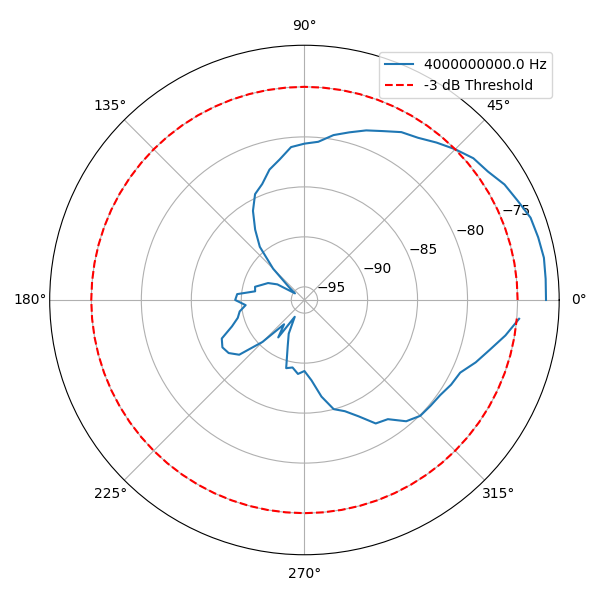
\includegraphics[width=0.8\linewidth]{./data/day5/polar_plot_4GHz.png}
    \caption{4GHzにおける放射パターン (極座標プロット)}
    \label{fig:polar_4GHz}
\end{figure}

\begin{figure}[h]
    \centering
    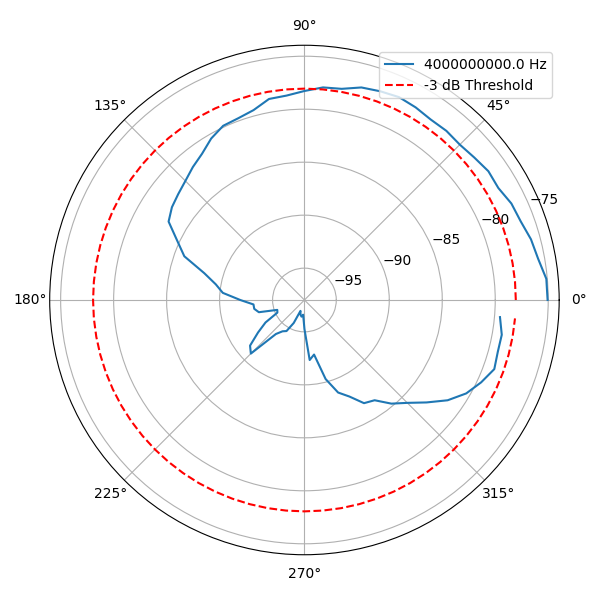
\includegraphics[width=0.8\linewidth]{./data/day5/polar_plot_8GHz.png}
    \caption{8GHzにおける放射パターン (極座標プロット)}
    \label{fig:polar_8GHz}
\end{figure}

\section{(5) 興味深い結果や事象について}
実験期間中, パッチアンテナが他の無線機器からの電波を受信する現象が観測された. この事象は, アンテナの設計周波数帯外の電波にも感度があることを示している. 特に実験室内で動作している無線LAN (2.4GHz, 5GHz帯) やBluetoothなどの信号が, アンテナを介して観測された可能性が高い. これらの信号は設計したアンテナの動作周波数とは異なるため, その影響を測定値から排除する必要があった.

シールド環境が使用されていない場合, 周囲の無線信号がアンテナに影響を与え, 設計した特性評価を妨げる可能性がある. このような影響を排除するためには, 無響室などのシールド環境を使用することが重要である. 一方で, 他の無線信号を受信する現象は, パッチアンテナが意図した動作周波数帯以外でも動作する能力を持つことを示しており, 受信用アンテナとしての応用可能性を示唆している.

\begin{figure}[h]
    \centering
    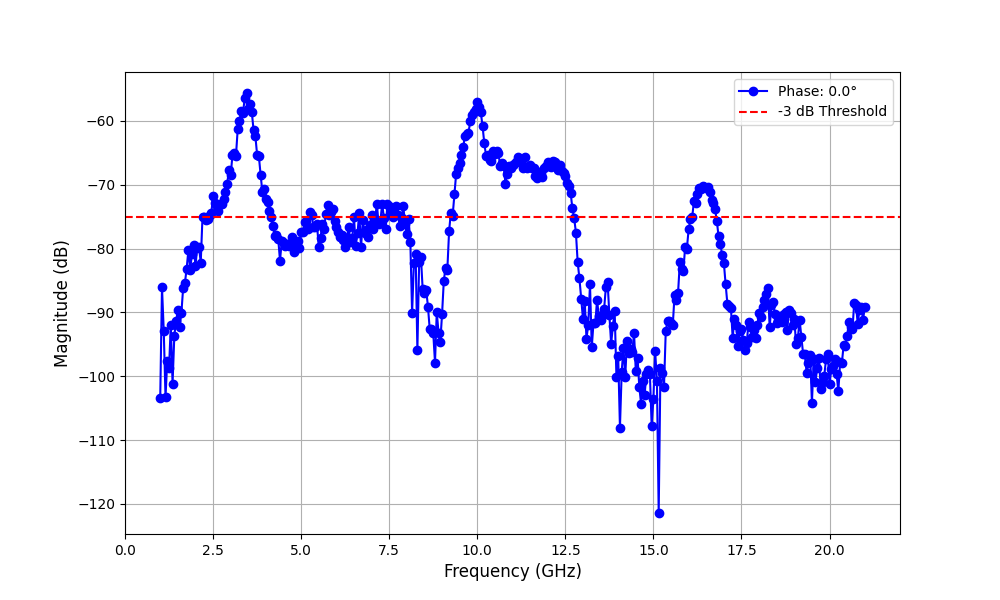
\includegraphics[width=0.8\linewidth]{./data/day5/line_plot_phase_0deg_4GHz.png}
    \caption{4GHzにおける位相 \(0^\circ\) の振幅特性}
    \label{fig:line_4GHz}
\end{figure}

\begin{figure}[h]
    \centering
    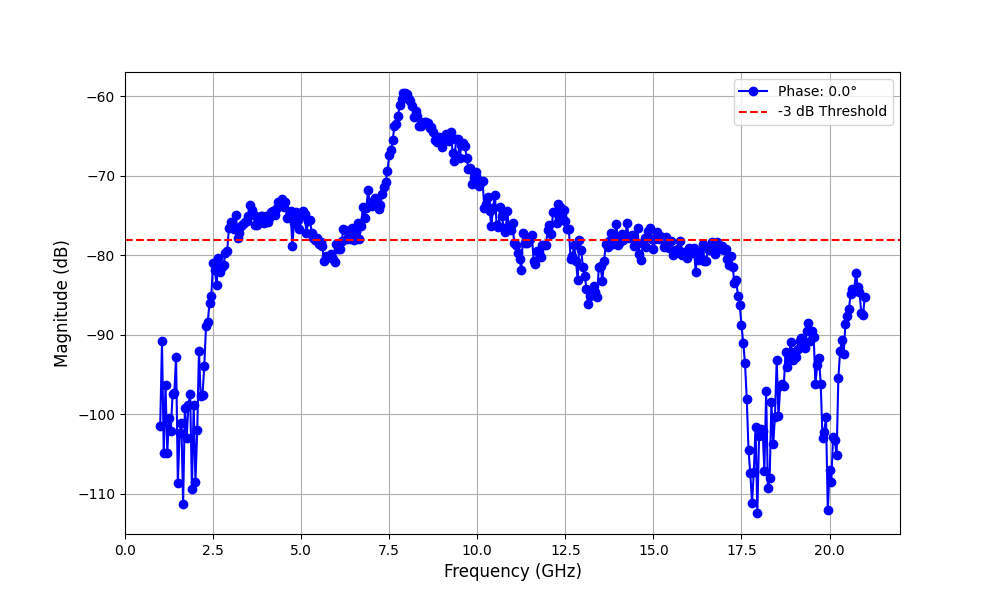
\includegraphics[width=0.8\linewidth]{./data/day5/line_plot_phase_0deg_8GHz.png}
    \caption{8GHzにおける位相 \(0^\circ\) の振幅特性}
    \label{fig:line_8GHz}
\end{figure}

以上より, パッチアンテナの放射パターンは設計寸法や周波数特性に基づいて形成される一方で, 実験環境や周囲の無線信号の影響を受けることが分かった. これらの影響を排除するためには, 測定環境の改善やシールド技術の導入が有効である.



\end{document}

